\documentclass[10pt,a4paper,twocolumn]{article}
\usepackage[left=3cm,right=2cm,top=2cm,bottom=2cm]{geometry}
\usepackage[utf8]{inputenc}
\usepackage[portuguese]{babel}
\usepackage[T1]{fontenc}
\usepackage{amsmath}
\usepackage{amsfonts}
\usepackage{amssymb}
\usepackage{graphicx}
\usepackage{hyperref}
\usepackage{times}

\title{\LARGE \bf
USO DE \textit{CONVERSATIONAL USER INTERFACE} PARA CONTROLE DE IoT
}

\author{\it
Alexandre Koslinski Neto$^{1}$, 
Giuliano Araujo Bertoti$^{2}$\\
$^{1,2}$FATEC São José dos Campos\\
\href{mailto:alexandre.koslinski@fatec.sp.gov.br}{alexandre.koslinski@fatec.sp.gov.br}
\href{mailto: giuliano.bertoti@fatec.sp.gov.br}{ giuliano.bertoti@fatec.sp.gov.br}
}

\begin{document}
 \vspace{-8ex}
  \date{}
\maketitle

\section{\bf Introdução}

Com o cenário de interação com o usuário cada vez mais intuitivo e natural, as interfaces baseadas em conversações (CUI - \textit{Conversational user interface}), estão cada vez mais presente no uso diário, com isso mais dispositivos forneceram uma interfasse de interação por esse meio.

O objetivo deste trabalho é verificar a viabilidade e encontrar meios mais naturais e intuitivos para interação entre o ser humano e dispositivos de IoT.

\section{\bf Materiais e Métodos}

Para facilitar o desenvolvimento o projeto foi separado em duas partes, um que aborda o \textit{chatbot} e outro o dispositivo que vai controlar a casa.
Esses dois contextos devem funcionar de forma independente.
\subsection{contexto do bot}
Para o desenvolvimento do teste, foi escolhido a plataforma de \textit{chatbot} do Telegram\cite{telegram}, tanto pela documentação disponível quanto pela facilidade de desenvolvimento. A linguagem utilizada para a implementação do \textit{chatbot} foi o Java, junto com o gerenciamento de dependências, Maven.

\subsection{contexto do IoT}
\subsubsection{\textit{Hardware}}
O dispositivo utilizado foi o \textbf{esp8266}\cite{esp}, pela capacidade de conexão via \textit{WiFi}. Tambem foram utilizados LEDs e resistores para a representação da comunicação entre \textit{chatbot} e dispositivo de IoT.

\subsubsection{\textit{Software}}
Para a programação do esp8266, foi utlilizado a linguagem de programação do arduino.

\section{\bf Resultados}
Como objeto de estudo foi iniciado o desenvolvimento para interação entre homem e dispositivo de IoT(\textit{Internet of Things}), como meio de facilitar a utilização e verificar a viabilidade desse metodo.


O usuario pergunta ou faz algum comando, atualmente, apenas por texto, para o \textit{chatbot}. O comando é interpretado e dado o devido comando para o dispositivo IoT.


O dispositivo IoT possue um servidor configurado, que recebe requisições e executa uma função ou conjunto de funções a partir do serviço requisitado.


A resposta do usuario é a ação realizada com sucesso ou uma mensagem alertando da impossibilidade dessa ação.


 
\begin{figure}[h]
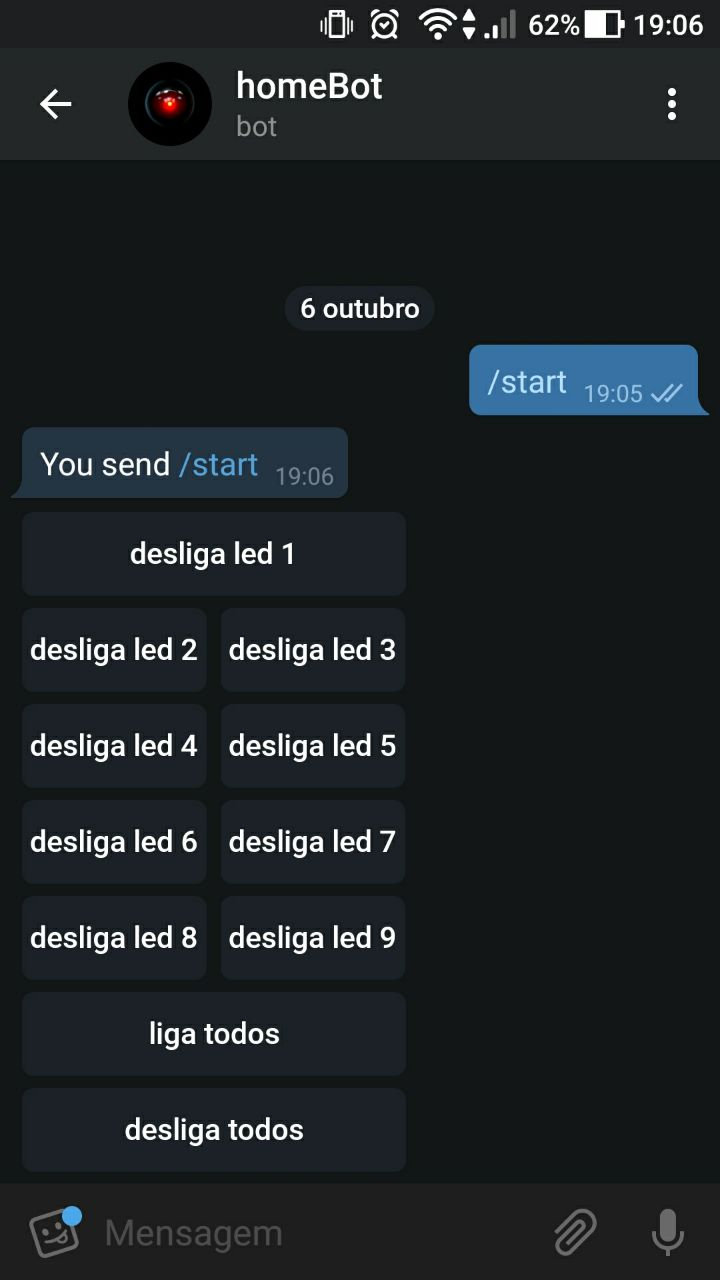
\includegraphics[scale=0.1]{img-1}
\caption{Demonstração de uso.}
\end{figure}


\section{\bf Conclusões}
Após o desenvolvimento e teste. Foi verificado a possibilidade de uma interface de comunicação entre um dispositivo de  IoT e o Telegram. Foi comprovado a viabilidade de um sistema do tipo. Além disso, foi verificado que um processamento de linguagem natural pode facilitar a interação entre os dispositivos.

 Link para o \textit{github}: \url{https://github.com/alexNeto/smart-home-bot}
%\href{https://github.com/alexNeto/smart-home-bot}{Link para o \textit{github}}


\begin{thebibliography}{99}
\bibitem{telegram}  \url{https://telegram.org/}
\href{https://telegram.org/}{Aplicativo de conversação que facilita o desenvolvimento de chatBots}
\bibitem{esp} \url{https://cdn-shop.adafruit.com/product-files/2471/0A-ESP8266__Datasheet__EN_v4.3.pdf}
\href{https://cdn-shop.adafruit.com/product-files/2471/0A-ESP8266__Datasheet__EN_v4.3.pdf}{Dispositivo para IoT, conecção \textit{wireless}} 
\end{thebibliography}

\end{document}